\subsection{Goal Ordering}
\label{subsec:disc_goal_ordering}

As shown in \cref{sec:results}, our goal prioritisation algorithm enables us to solve 16 out of the 30 given solvable levels. 
It is however important in this discussion segment to stress some of the flaws that come with our algorithm. 
In this subsection we'll outline some of the strengths and weaknesses found in our goal prioritisation. 

\subsubsection{Strengths} From the competition we learned that our client was succesfully able to prioritise goals in levels such as \texttt{MAteamhal}. 
This level includes one opening which branches into two different one-way paths, as can be seen in the included \cref{fig:mateamhal}.
This can be attributed to the fact that our ordering algorithm increments the opening of the goals (in this case the middle), for each iteration of the scoring matrix (see \cref{methods:goal_ordering}). 
As such the opening in the middle will get the heighest score, and therefore everything following will decrese. 
With this technique, we are able to solve both problems like \texttt{MAteamhal}, as well as levels with different groups of goals. 

\begin{figure}[h!]
  \centering
  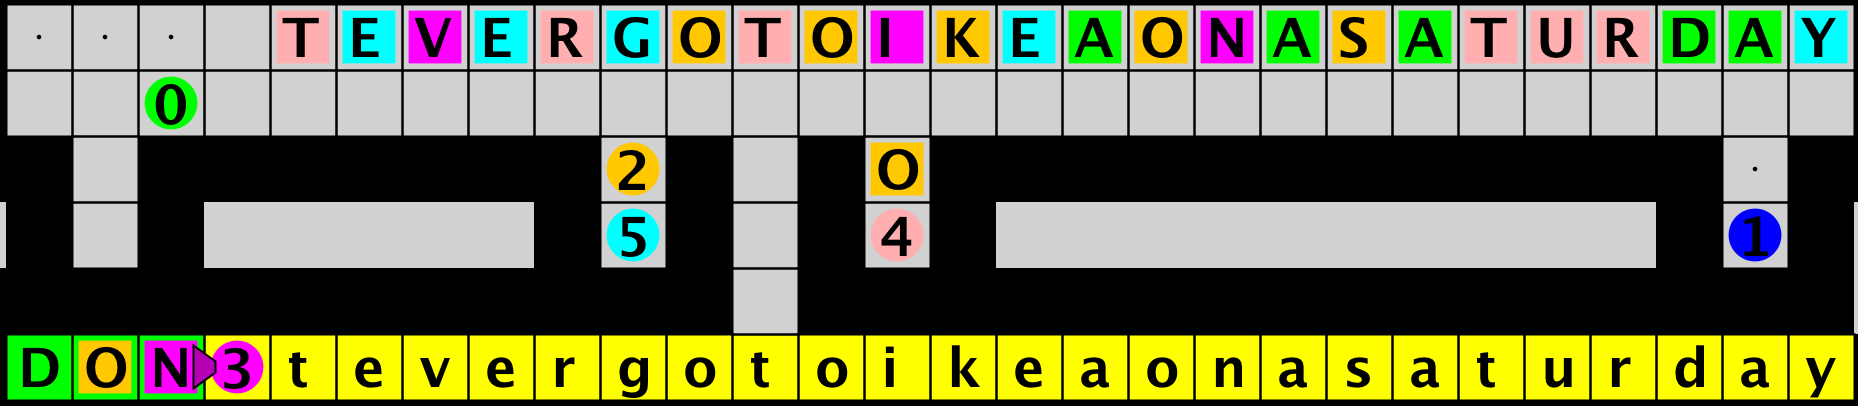
\includegraphics[width=.7\columnwidth]{graphics/mateahhal.png}
  \caption{\label{fig:mateamhal}Our client solving MAteamhal}
\end{figure}

\subsubsection{Weaknesses} Defining the opening (or entrance) to a group of goals as the goal with the most neighbouring free cells, does have it issues however. 
While working great in cases such as the one seen in \cref{fig:mateamhal}, problems arise if the entrance to a group of goals is not actually the goal with the heighest number of neighbouring free cells. 
An example of this can be found in \cref{fig:examplelev}.
Here we see that goal \textbf{c} has the heighest number of neighboring free cells, and as such, our ordering algorithm will find it to be blocking the other goals, even though it is not. 
In the class competition, we did not encounter a problem like this, however the problem is indeed a known weakness of our prioritisation algorithm.

\begin{figure}[h!]
  \centering
  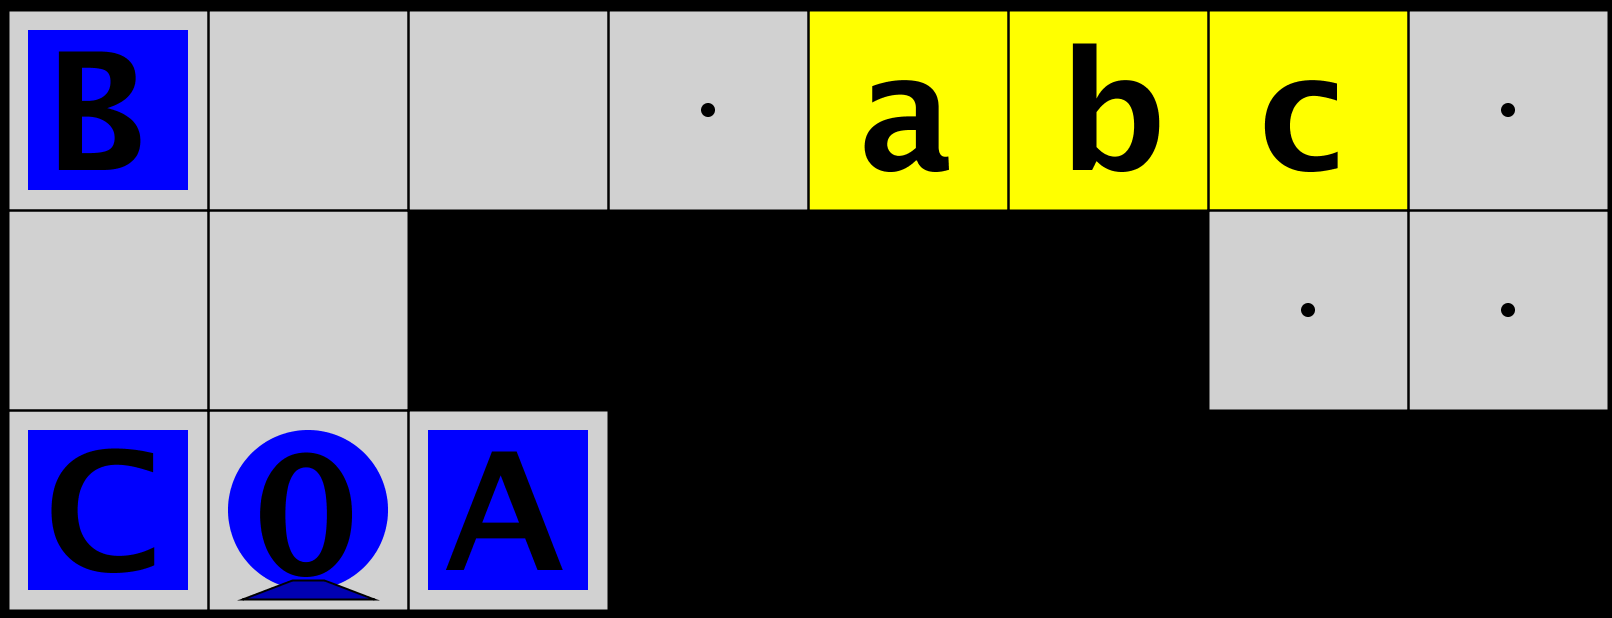
\includegraphics[width=.6\columnwidth]{graphics/ordering_issue.png}
  \caption{\label{fig:examplelev}Example level}
\end{figure}
 